% !TeX spellcheck = pl_PL
\documentclass[a4paper,11pt]{article}

\usepackage{fullpage}
\usepackage{polski}
\usepackage[T1]{fontenc}
\usepackage[utf8]{inputenc}
\usepackage{times}

\usepackage{amssymb}
\usepackage{amsmath}
\usepackage{textcomp}
\usepackage{graphicx}

\usepackage{hyperref}
\hypersetup{hidelinks}
\urlstyle{same} 

\usepackage{dsfont}
\newcommand{\bra}[1]{\left\langle{#1}\right|}
\newcommand{\ket}[1]{\left|{#1}\right\rangle}
\newcommand{\braket}[2]{\left\langle{#1}|{#2}\right\rangle}
\newcommand{\ketbra}[2]{\left| #1 \right\rangle \left\langle#2\right|}
\newcommand{\Id}{\mathds{I}}

\newcommand{\ang}[1]{(ang. \emph{#1})}


\begin{document}


\title{Kwantowe obliczenia wariacyjne\\ {\normalsize Przegląd wybranych zastosowań}}

\author{Jarosław Miszczak}
\date{29/12/2022}

\maketitle

\begin{abstract}
Raport przedstawia wybrane zastosowania wariacyjnych algorytmów kwantowych. Przedstawione są proponowane algorytmy wariacyjne które mogą być wykorzystywane do estymacji energii stanu podstawowego, rozwiązywania problemów optymalizacji kombinatorycznej oraz problemów pojawiających się w informatyce kwantowej.
\end{abstract}

\tableofcontents

\newpage


%-------------------------------------------------------------------------------
\hypertarget{wprowadzenie}{%
\section{Wprowadzenie}\label{wprowadzenie}}
%-------------------------------------------------------------------------------

W ostatnich kilku dekadach badacze z wielu obszarów nauki i techniki połączyło siły w celu zbadania i opracowania algorytmów kwantowych oraz ich eksperymentalnej realizacji. Jednak większość pierwotnie zaproponowanych algorytmów kwantowych wymaga milionów fizycznych qubitów do implementacji na sprzęcie kwantowym. Istniejący sprzęt kwantowy zawiera bardzo mało (rzędu stu) fizycznych qubitów i są one nazywane urządzeniami Noisy Intermediate-Scale Quantum (NISQ). Wariacyjne algorytmy kwantowe (VQAs) są klasą algorytmów NISQ, które mogą być zaimplementowane na urządzeniach NISQ i zostały zaprojektowane biorąc pod uwagę ograniczenia tej klasy urządzeń.

\begin{figure}[ht!]
	\centering
	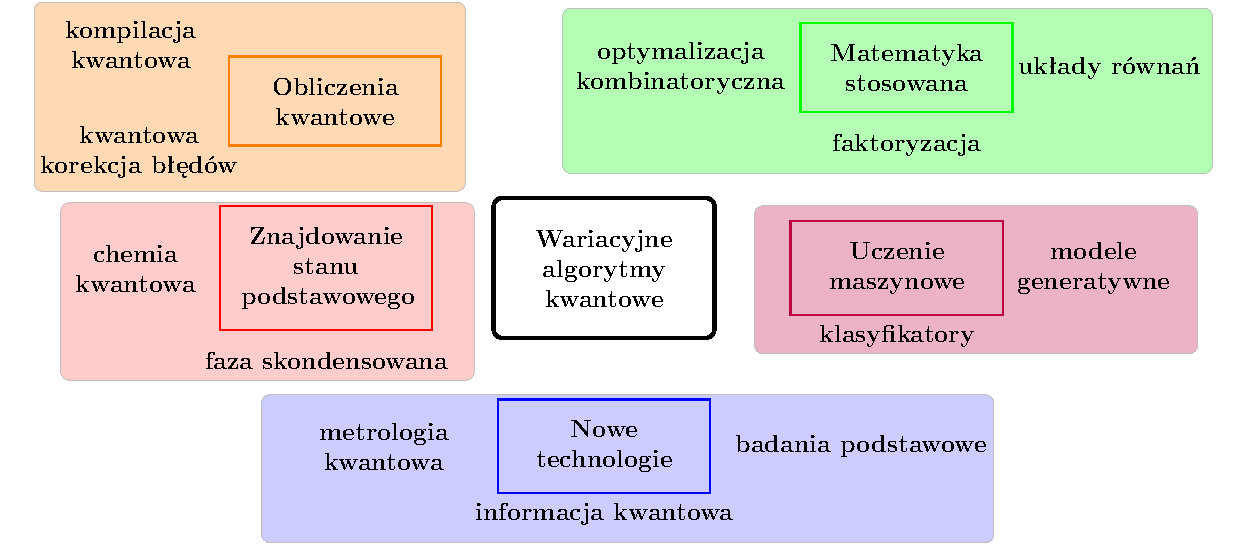
\includegraphics[width=\textwidth]{vqa-applications-pl}
	\caption{Potencjalne dziedziny w których zastosowanie wariacyjnych algorytmów kwantowych może prowadzić do uzyskania przewagi kwantowej.}
\end{figure}

Wśród klasy VQAs, Variational Quantum Eigensolver (VQE) pomaga nam znaleźć stan podstawowy cząsteczki. Ma to zastosowanie w odkrywaniu leków, materiałoznawstwie i chemii kwantowej. Innym przykładem VQA jest kwantowy przybliżony algorytm optymalizacji (QAOA), który może być używany do kodowania i rozwiązywania binarnych problemów optymalizacyjnych.

Pierwszym i jednocześnie najbardziej rozpowszechnionym zastosowaniem VQA jest estymacja stanów podstawowych i odpowiadających im wartości własnych energii dla zadanego Hamiltonianu. Algorytmy kwantowe dla znajdowania stanu podstawowego danego Hamiltonianu projektowane dla uniwersalnych komputerów kwantowych opierały się na adiabatycznym przygotowaniu stanu i podprogramach kwantowej estymacji fazy. Niestety wymagania tych algorytmów dotyczące głębokości obwodu przekraczają te dostępne w erze NISQ.


Poza statycznymi problemami stanów własnych, VQA mogą być również stosowane do symulacji dynamicznej ewolucji układu kwantowego. Konwencjonalne algorytmy symulacji Hamiltonianu kwantowego, takie jak formuła produktu Trottera-Suzuki,  dyskretyzują czas na małe kroki i symulują każdą ewolucję czasową za pomocą obwodu kwantowego. Dlatego głębokość obwodu zazwyczaj rośnie wielomianowo z rozmiarem systemu i symulowanym czasem.

Natomiast pierwszą grupą procedur kwantowych służących do optymalizacji są algorytmy bazujące na QAOA (Quantum Approximate Optimization Algorithm) -- algorytmach przybliżonej optymalizacji kwantowej. Algorytm te to heurystyki do projektowania wariacyjnych układów bramek do optymalizacji kombinatorycznej. Schemat ten opiera się na wykorzystaniu twierdzenia adiabatycznego. Zadanie optymalizacji kombinatorycznej ma na celu znalezienie optymalnego obiektu z skończonego zbioru rozwiązań. Problem można sformułować jako maksymalizację funkcji celu, która jest sumą funkcji boolowskich.
Na potrzeby realizacji procedury optymalizacyjnej na komputerze kwantowym funkcja celu reprezentowana jest jako model QUBO (Quandratic Unconstrained Binary Optimization). W modelu takim dopuszcza się tylko zmienne binarne i mogą występować one w wyrazach drugiego rzędu.

Zarówno VAE jak i QAOA są kwantowo-klasycznymi algorytmami, których zasadniczą częścią jest układ bramek kwantowych wykonywany na sprzęcie kwantowym. Układ ten jest często reprezentowany przez serię sparametryzowanych jednokubitowych i nieparametryzowanych dwukubitowych kwantowych bramek logicznych. W ten sposób przygotowany zostaje stan kwantowy. Następnie energia układu którego cechy chcemy zbadać jest optymalizowana na klasycznym komputerze w celu uzyskania energii stanu podstawowego. 

Jednym z najtrudniejszych aspektów VQA jest skonstruowanie efektywnego układu bramek kwantowych. Wydajność tego układu jest definiowana przez określenie:
\begin{itemize}
\item jak mała jest głębokość, gdzie każda warstwa zawiera tylko równoległe operacje, układu bramek, 
\item dokładność w oszacowaniu energii stanu podstawowego, oraz 
\item ocenę funkcji energii na klasyczny przebieg optymalizacji.
\end{itemize}




\newpage


%-------------------------------------------------------------------------------
\section{Obliczenia kwantowe}
%-------------------------------------------------------------------------------
\newpage
%-------------------------------------------------------------------------------
\subsection{Kompilacja kwantowa}
%-------------------------------------------------------------------------------
\newpage
%-------------------------------------------------------------------------------
\subsection{Kwantowa korekcja błędów}
%-------------------------------------------------------------------------------

\newpage
%-------------------------------------------------------------------------------
\section{Znajdowanie stanu podstawowego}
%-------------------------------------------------------------------------------

Pierwszym i jednocześnie najbardziej rozpowszechnionym zastosowaniem VQA jest estymacja stanów podstawowych i odpowiadających im wartości własnych energii dla zadanego Hamiltonianu. Algorytmy kwantowe dla znajdowania stanu podstawowego danego Hamiltonianu projektowane dla uniwersalnych komputerów kwantowych opierały się na adiabatycznym przygotowaniu stanu i podprogramach kwantowej estymacji fazy. Niestety wymagania tych algorytmów dotyczące głębokości obwodu przekraczają te dostępne w erze NISQ.


Z tego powodu pierwszy zaproponowany kwantowy algorytm wariacyjny, Variational Quantum Eigensolver (VQE), został opracowany w celu zapewnienia przybliżonego rozwiązania tego zadania.  W tym miejscu dokonujemy przeglądu zarówno oryginalnej architektury VQE, jak i niektórych bardziej zaawansowanych metod znajdowania stanów podstawowych i wzbudzonych. 


%-------------------------------------------------------------------------------
\subsection{Chemia kwantowa}
%-------------------------------------------------------------------------------
\newpage

%-------------------------------------------------------------------------------
\subsection{Fizyka fazy skondensowanej}
%-------------------------------------------------------------------------------

Poza statycznymi problemami stanów własnych, VQA mogą być również stosowane do symulacji dynamicznej ewolucji układu kwantowego. Konwencjonalne algorytmy symulacji Hamiltonianu kwantowego, takie jak formuła produktu Trottera-Suzuki,  dyskretyzują czas na małe kroki i symulują każdą ewolucję czasową za pomocą obwodu kwantowego. Dlatego głębokość obwodu zazwyczaj rośnie wielomianowo z rozmiarem systemu i symulowanym czasem.

Biorąc pod uwagę szum nieodłącznie związany z urządzeniami NISQ, skumulowane błędy sprzętowe dla takich głębokich obwodów kwantowych mogą okazać się zaporowe. Aby rozwiązać ten problem, VQA do dynamicznej symulacji kwantowej używają tylko płytkiego obwodu głębokości, znacznie zmniejszając wpływ szumu sprzętowego.


Ramy VQA można również rozszerzyć do symulacji dynamicznej ewolucji otwartych układów kwantowych. 
 
 
 
% Przypuśćmy, że dynamika układu opisana jest przez $\frac{\rho}{dt} = \mathcal{L}{\rho)$, gdzie $\mathcal{L}$ oznacza superoperator dla procesu dyssypatywnego. Podobnie jak w podejściu iteracyjnym dla stanów czystych~, odwzorowuje się ewolucję stanu mieszanego na jeden z parametrów wariacyjnych poprzez zasadę McLachlana, która rozwiązuje minimalizację $min_{dot{theta}}|(\frac{d}{dt}- \mathcal{L})\rho(\i0)$. Rozwiązanie określa ewolucję parametrów $ M_{i,j}}= V$ przy czym 
%
% $M_{i,j}= ^mathrm{Tr}}}}big[^partial_i ^rho(vec{theta})^dag ^partial_j^rho(vec{theta}) ^big]$,  


Każdy człon $M$ i $V$ może być obliczony przez zastosowanie układu testowego 
SWAP na dwóch kopiach stanów oczyszczonych~. Tutaj, aby zasymulować otwarty układ $n$ qubitów, należy zastosować operacje na $4n+1$ qubitach. Alternatywnym podejściem, które zmniejsza ten narzut, jest symulacja stochastycznego równania Schr\"odingera, które rozkłada ewolucję macierzy gęstości na trajektorie czystych stanów. Każda trajektoria czystego stanu doświadcza ciągłego efektu tłumienia i procesów skokowych spowodowanych operatorami szumu, z których oba mogą być efektywnie symulowane. Ponieważ w tej metodzie kontroluje się tylko jedną kopię stanu czystego, wymaga ona jedynie $n+1$ qubitów. 

\newpage
\ 
\newpage

%-------------------------------------------------------------------------------
\section{Nowe technologie}
%-------------------------------------------------------------------------------

\newpage
%-------------------------------------------------------------------------------
\subsection{Metrologia kwantowa}
%-------------------------------------------------------------------------------
\newpage
%-------------------------------------------------------------------------------
\subsection{Informacja kwantowa}
%-------------------------------------------------------------------------------

\paragraph{Kompilacja obwodów kwantowych} Kompilacja algorytmów kwantowych dla komputerów kwantowych najbliższej przyszłości, uwzględniająca architekturę połączeń oraz dostępne operacje natywne jest sporym wyzwaniem. Uniknięcie wykładniczego narzutu klasycznej symulacji dynamiki kwantowej pozwoli na kompilację większych algorytmów, a strategią na to jest ocena kosztu algorytmu na komputerze kwantowym. W tym celu proponujemy wariacyjny hybrydowy algorytm kwantowo-klasyczny zwany kwantowo wspomaganą kompilacją (QAQC -- Quantum Assistaed Quantum Compilation). 
%
W QAQC funkcją kosztu jest iloczyn skalarny docelowej operacji unitarnej $U$ i trenowanej operacji unitarnej $V$ określony jako $tr U^\dagger V$. Tak jak we wszystkich VQA funkcja ta jest ewaluowana za pomocą obwodu kwantowego.
%
Aby zapewnić, że QAQC dobrze skaluje się z wielkością problemu, zaproponowany koszt obejmuje nie tylko globalne nakładanie się operacji, ale także lokalne nakładanie się w odniesieniu do poszczególnych qubitów. Dzięki temu możliwe możliwe było zaproponowanie płytkich obwodów kwantowych. Wykazano również, że wprowadzony koszt nie nie może być efektywnie przybliżony klasycznym algorytmem przy rozsądnych założeniach złożoności.
% 
Zastosowania QAQC obejmują kompresję głębokości algorytmów, kompilację czarnej skrzynki, motywację błędów i benchmarking.
\newpage
%-------------------------------------------------------------------------------
\subsection{Badania podstawowe}
%-------------------------------------------------------------------------------


\newpage
\ 
\newpage

%-------------------------------------------------------------------------------
\section{Uczenie maszynowe}
%-------------------------------------------------------------------------------
\newpage
%-------------------------------------------------------------------------------
\subsection{Klasyfikatory}
%-------------------------------------------------------------------------------
\newpage

%-------------------------------------------------------------------------------
\subsection{Modele generatywne}
%-------------------------------------------------------------------------------
\newpage
\ 
\newpage

%-------------------------------------------------------------------------------
\section{Matematyka stosowana}
%-------------------------------------------------------------------------------
\newpage
%-------------------------------------------------------------------------------
\subsection{Rozwiązywanie układów równań}
%-------------------------------------------------------------------------------
\newpage
%-------------------------------------------------------------------------------
\subsection{Optymalizacja kombinatoryczna}
%-------------------------------------------------------------------------------

Pierwszą grupą procedur kwantowych służących do optymalizacji są algorytmy bazujące na QAOA (Quantum Approximate Optimization Algorithm) -- algorytmach przybliżonej optymalizacji kwantowej. Algorytm te to heurystyki do projektowania wariacyjnych układów bramek do optymalizacji kombinatorycznej. Schemat ten opiera się na wykorzystaniu twierdzenia adiabatycznego.


Zadanie optymalizacji kombinatorycznej ma na celu znalezienie optymalnego obiektu z skończonego zbioru rozwiązań. Problem można sformułować jako maksymalizację funkcji celu, która jest sumą funkcji boolowskich.

Każda funkcja logiczna $C_\alpha:\{0,1\}^n\rightarrow\{0,1\}$ przyjmuje na wejściu ciąg 0-1, a zwraca jedną z wartości 0 lub 1. Problem optymalizacji kombinatorycznej na $n$ bitach i $m$ klauzulach jest równoważny znalezieniu ciągu bitów który maksymalizuje funkcję
\[
C (z) = \sum_{\alpha = 1}^m C_\alpha(z), \quad z\in\{0,1\}^n
\] 

Na potrzeby realizacji procedury optymalizacyjnej na komputerze kwantowym funkcja celu reprezentowana jest jako model QUBO (Quandratic Unconstrained Binary Optimization). W modelu takim dopuszcza się tylko zmienne binarne i mogą występować one w wyrazach drugiego rzędu,
\[
C_{QUBO}(b) = \sum_{i\leq j}w_{ij} b_i b_j,
\]
gdzie macierz $w_{ij}\in\mathds{R}$ reprezentuje wagi. Maksymalizacja  $C_{QUBO}(b)$ odpowiada znalezieniu ciągu bitów $b = b_1b_2\dots b_n$

Na bazie modelu QUBO problemu możliwe jest zapisanie Hamiltoniamu modelu Isinga odpowiadającego temu problemowi. W tym celu każdej zmiennej binarnej $b_i$ przyporządkowuje się operator $Z_i$ odpowiadający macierzy Pauliego Z działającej na $i$-ty spin,
\[
b_i \mapsto \frac{1}{2}(1-Z_i).
\]
W ten sposób Hamiltonian funkcji celu przyjmuje postać
\[
H_C = \sum_{i\leq j} w_{ij} (1-Z_i)(1- Z_j),
\]
co powoduje, iż w modelu występują jedynie oddziaływania dwucząstkowe. 

Hamiltionain $H_0$ jest budowany z macierzy Pauliego X
\[
H_0 = \sum_i X_i,
\]
a stan początkowy jest stanem własnym $H_0$. 

\begin{figure}
	\begin{center}
		\includegraphics{qaoa-pl.pdf}
		\caption{Schemat działania kwantowego algorytmu przybliżonej optymalizacji. Para kątów $\gamma_k,\eta_k$, reprezentująca czas ewolucji dla $H_C$ i $H_0$, jest dobierana dla każdej iteracji w taki sposób aby wykonanie obwodu doprowadziło do minimalizacji funkcji kosztu zdefiniowanej przez $H_C$.}
	\end{center}
\end{figure}

Obwody kwantowe konstruowane tą metodą składają się z naprzemiennego stosowanie bloku funkcji celu i bloku ewolucji. Stan układu po wykonaniu $k$ iteracji jest postaci
\[
\ket{\phi_k(\gamma,\eta)} = e^{-i\eta_k H_O} e^{-i\gamma_k H_C}\dots e^{-i\eta_1 H_O}e^{-i\gamma_k H_C}\left(\frac{\ket{0}+\ket{1}}{2}\right)^n.
\]
Hamiltonian ten odpowiada serii obrotów $R_X$, natomiast $H_C$ odpowiada obrotom $R_Z$. 


Przykładowo, rozważmy problem podziału: czy dla $S=\{n_1,\dots,n_N\}$ istnieje taki podział na dwa zbiory $R$ oraz $S \setminus R$ takie, że
\[
\sum_{R}n_i = \sum_{S\setminus R} n_i.
\]
Dla takiego problemu
\[
H_C = \sum_{i=1}^N n_i Z_i.
\]
Jeżeli istnieje stan podstawowy $H_C$ z energią równą 0, to oznacza, iż istnieje konfiguracja spinów w stanie $+1$ i w stanie $-1$, taka, że odpowiednie sumy $n_i$ się znoszą.

\newpage
\ 
\newpage

\hypertarget{literatura}{%
\section*{Literatura}\label{literatura}}

\begin{enumerate}
\def\labelenumi{\arabic{enumi}.}
%\tightlist


\subsection*{Znajdowanie stanu podstawowego}

\item Aspuru-Guzik, A., Dutoi, A.D., Love, P.J. and Head-Gordon, M., 2005. Simulated quantum computation of molecular energies. Science, 309(5741), pp.1704-1707.

\item Abrams, D.S. and Lloyd, S., 1999. Quantum algorithm providing exponential speed increase for finding eigenvalues and eigenvectors. Physical Review Letters, 83(24), p.5162.


\subsection*{Obliczenia kwantowe}

\item Khatri, S., LaRose, R., Poremba, A., Cincio, L., Sornborger, A.T. and Coles, P.J., 2019. Quantum-assisted quantum compiling. Quantum, 3, p.140. \url{https://arxiv.org/abs/1807.00800} \url{https://doi.org/10.22331/q-2019-05-13-140}

\subsection*{Rozwiązywanie układów równań}

\item Huang, H.Y., Bharti, K. and Rebentrost, P., 2021. Near-term quantum algorithms for linear systems of equations with regression loss functions. New Journal of Physics, 23(11), p.113021. \url{https://doi.org/10.1088/1367-2630/ac325f}


\item Bravo-Prieto, C., LaRose, R., Cerezo, M., Subasi, Y., Cincio, L. and Coles, P.J., 2019. Variational quantum linear solver. LA-UR-19-29101, arXiv:1909.05820. \url{https://doi.org/10.48550/arXiv.1909.05820}

\item Pellow-Jarman, A., Sinayskiy, I., Pillay, A. et al. A comparison of various classical optimizers for a variational quantum linear solver. Quantum Inf Process 20, 202 (2021). \url{https://doi.org/10.1007/s11128-021-03140-x}



\end{enumerate}

\end{document}
